\chapter{Games and emotions}

Research about games is a broad topic that involves different disciplines and definitions. In the context of this thesis, a game is defined as a system in which players engage in an artificial conflict, defined by rules, that results in a goal \parencite{salen2004rules}. An artificial conflict is a set of challenges that the player must overcome towards the game goal, e.g. sort elements within a time constraint.

\textcite{schell2014art} mentions that, from a game design perspective, the difficulty level of such challenges affects the emotional state of players, e.g. moments of boredom or anxiety/stress. Every time a reward is given to the player, which usually is a tool to increase the player's power, the game's challenge level is lowered because the player becomes stronger. After a period, such increase in the player's skill level causes the game to be boring because the challenges are now easier to beat. At that point, the difficulty level is again increased by the game, raising the challenging levels for the player once more, causing anxiety. The anxiety and stress period lasts until the player is rewarded again, when the newly obtained power will eventually lower the challenge levels again (resulting in boredom), causing the cycle to repeat itself. A challenge beyond the player's skill to address and overcome it causes anxiety, while the opposite results in disinterest, leading to boredom \parencite{chen2007flow}. An ideal challenge/skill balance in a repeating cycle of increasing challenge followed by a reward keeps the player in an optimal experience and concentration state called flow \parencite{csikszentmihalyi1991flow}, as illustrated by Figure \ref{fig:flow-schell}.

\begin{figure}[h!]
    \centering
    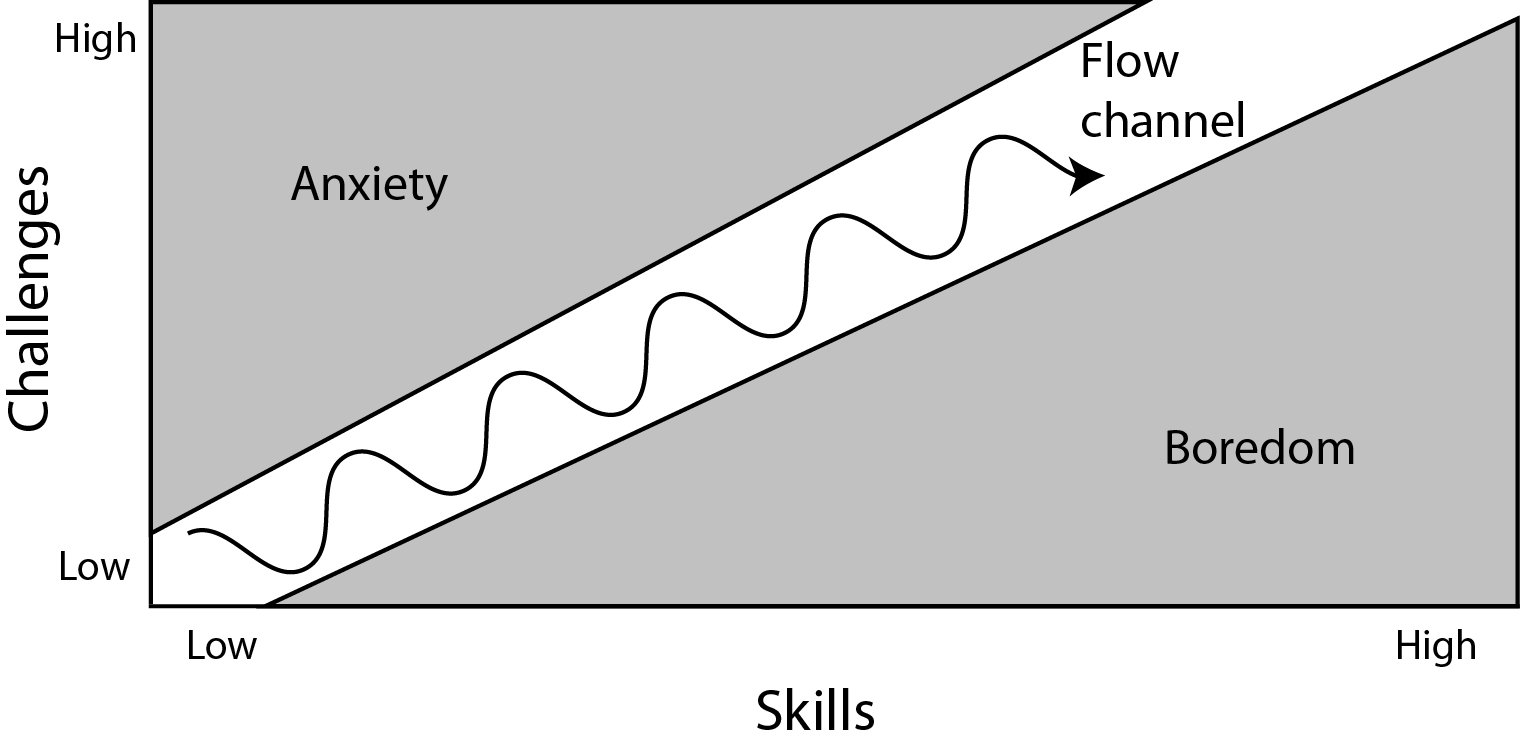
\includegraphics[scale=0.8]{figures/flow-schell.png}
    \caption{Repeating cycle of increasing challenge followed by a reward, keeping the player in the flow zone. \parencite{schell2014art}}
    \label{fig:flow-schell}
\end{figure}

The Theory of Flow is vastly mentioned in the literature, including its connection to engagement/immersion \parencite{brown2004grounded}, sense of presence \parencite{weibel2011immersion} and applicability in game design \parencite{cruz2017player, sweetser2005gameflow}. The following sections describe in more detail the theoretical foundation of emotions, connecting them to the context of games.

%%%%%%%%%%%%%%%%%%%%%%%%%%%%%%%%%%%%%%%%%%%%%%%%%%%%%%%%%%%%%%%%%%%%%%%%%%%%%%%%%%%%%%%%%%%%%%%%%%%%%%%
\section{Emotions theory}
%%%%%%%%%%%%%%%%%%%%%%%%%%%%%%%%%%%%%%%%%%%%%%%%%%%%%%%%%%%%%%%%%%%%%%%%%%%%%%%%%%%%%%%%%%%%%%%%%%%%%%%

\textcite{csikszentmihalyi1991flow} defined as flow a phenonmenon in which a person experiences a subjective state characterized by an instense level of attention during the execution of an intrinsically motivated activity. As previously mentioned, an ideal challenge/skill balance in a game leads players to an optimal experience and concentration state (i.e. flow), so flow constructs are of interest to the games community. Such peculiar state of flow, however, is not limited to activities involving games, so it can be experienced in a variety of other activities, e.g. dancing and climbing. It is outside the scope of this thesis the connection of the Theory of Flow to contexts other than games.

Further research \parencite{nakamura2014concept} refined the original definition of the flow state, culminating in the eight channel model of flow, illustrated in Figure \ref{fig:flow-eight}. Such model better describes the emotional state of users according to the challenge/skill balance in relation to the subject mean, since it is less coarse then the original flow model. In the eight channel model of flow, for instance, a person performing a low skill and low challenging task experiences apathy, while in the original model the classification would indicate a flow state.

\begin{figure}[h!]
    \centering
    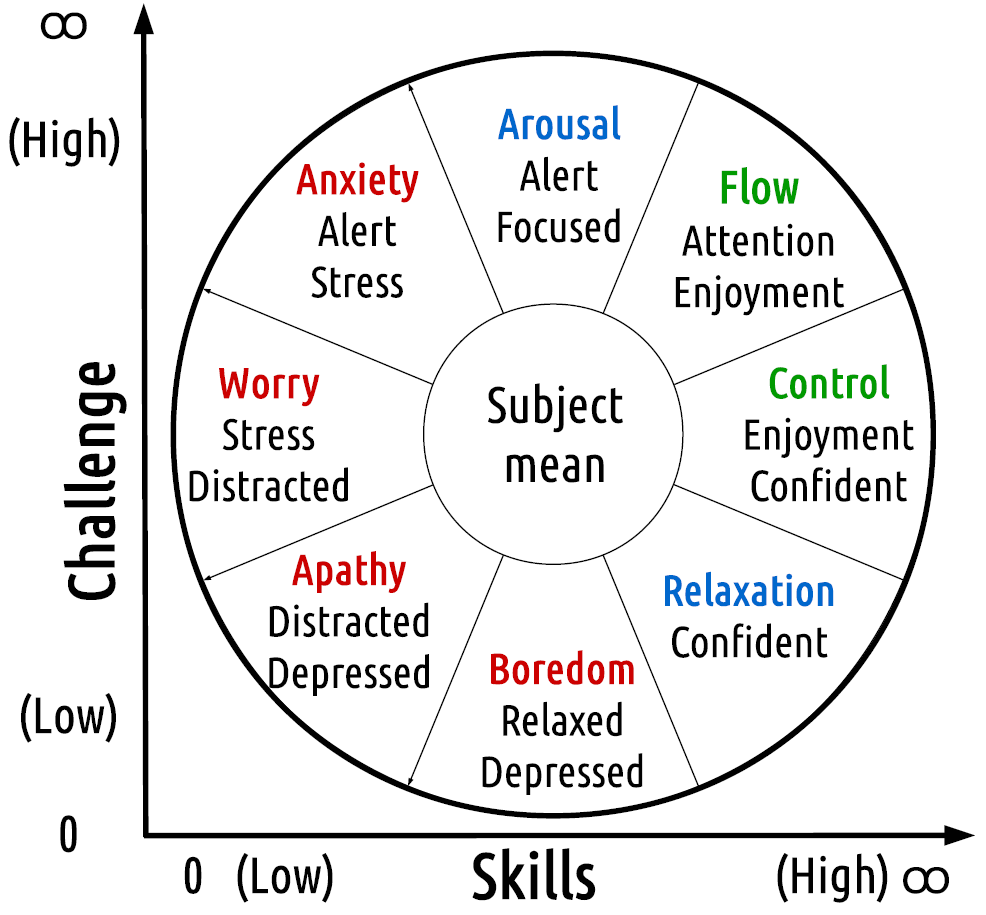
\includegraphics[scale=0.5]{figures/flow-eight.png}
    \caption{\parencite{nakamura2014concept}}
    \label{fig:flow-eight}
\end{figure}

%\subsection{Russell's AV dimensional theory of emotions}

\ref{fig:av-model}
\textcite{russell1978evidence}
\textcite{posner2005circumplex}

\begin{figure}[h!]
    \centering
    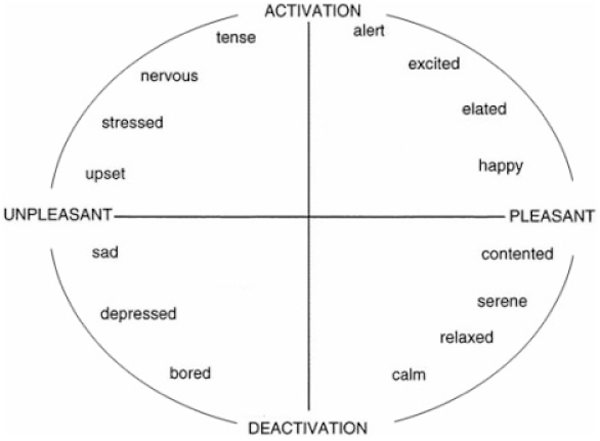
\includegraphics[scale=0.8]{figures/russell-av.png}
    \caption{Representation of the circumplex model of affect \parencite{posner2005circumplex}. Horizontal axis represents the valence dimension and the vertical axis represents the arousal or activation dimension.}
    \label{fig:av-model}
\end{figure}

%%%%%%%%%%%%%%%%%%%%%%%%%%%%%%%%%%%%%%%%%%%%%%%%%%%%%%%%%%%%%%%%%%%%%%%%%%%%%%%%%%%%%%%%%%%%%%%%%%%%%%%
\section{Stress, boredom and flow}
%%%%%%%%%%%%%%%%%%%%%%%%%%%%%%%%%%%%%%%%%%%%%%%%%%%%%%%%%%%%%%%%%%%%%%%%%%%%%%%%%%%%%%%%%%%%%%%%%%%%%%%




%%%%%%%%%%%%%%%%%%%%%%%%%%%%%%%%%%%%%%%%%%%%%%%%%%%%%%%%%%%%%%%%%%%%%%%%%%%%%%%%%%%%%%%%%%%%%%%%%%%%%%%
\section{Immersion, engagement and sense of presence}
%%%%%%%%%%%%%%%%%%%%%%%%%%%%%%%%%%%%%%%%%%%%%%%%%%%%%%%%%%%%%%%%%%%%%%%%%%%%%%%%%%%%%%%%%%%%%%%%%%%%%%%

The previously mentioned works try to relate physiological signals to emotional states. In games research, such initiatives are important to enhance the tooling available to better understand the player's experience while playing games. One concept that tries to model player experience is named flow, which was defined by \textcite{csikszentmihalyi1991flow}. Flow is an optimal experience achieved by the player during the interaction with a game. When in flow, a player will lose sense of time and space, focusing almost exclusively on the game being played, with a feeling of "being there".

The definition of flow, however, requires a more sophisticated interpretation, as investigated by further research. From a game design perspective, for instance, Schell \parencite{schell2014art} mentions that a progression of the player in the flow zone is desired, however it should not be a "straight line", but more of a cycle alternating among emotional states as stress, enjoyment and boredom. Different elements are connected to flow, such as engagement, immersion and sense of presence. Immersion, for instance, was defined by Brown and Cairns \parencite{brown2004grounded}, who used Grounded Theory to find it refers to the degree of involvement with a computer game. In that light, the authors theorized that a player will overcome barriers that limit his/her degree of involvement in immersion. After each barrier is broken, the sense of immersion deepens. The first barrier, for instance, is named engagement and it refers to the player willingness  to invest attention and energy to learn how to play the game. The concept of flow, as defined by Csikszentmihalyi, is an extreme state, which is only achieved when the player has overcame all previously mentioned barriers and is in a "total immersion" state. Such condition is rare to happen since it requires the highest level of attention from the player. As a consequence, engagement is more plausible and common during gaming experiences than flow.

The existence of several works \parencite{boyle2012engagement} related to understanding and defining what engagement/immersion is demonstrates the interest of researchers to broaden the view beyond flow alone. Presence, for instance, which describes the player's feeling of actually being in the game, is reported as an important aspect of engagement and immersion \parencite{weibel2011immersion}. Studies connected to training simulation \parencite{engstrom2016impact}, for instance, also indicate that contextualization (increasing the sense of presence) might affect immersion positively. Additionally to the intentions of understanding and defining engagement and immersion, studies also try to measure them. The majority of the approaches used for that are based on questionnaires, which are by nature subjectively answered by players. Additionally that approach usually breaks any sense of presence of the player since it requires a shift in attention away from the game, hence breaking or affecting the level of engagement/immersion as well. More quantitative approaches have been investigated to measure engagement, such as the use of physiological signals like HR \parencite{ravaja20051} and eye movement \parencite{jennett2008measuring}, for instance. The complexity in defining engagement and immersion is also reflected in the task of measuring it. Ravaja et al. \parencite{ravaja20051}, for instance, mentions the significant variation of physiological signals as an obstacle; signals increase during emotional arousal, but decrease in response to attention engagement, which makes the measurement of engagement a non-trivial process. It highlights the difficulties in correlating qualitative data to more abstract concepts as engagement, immersion and flow.

Research initiatives that help in the identification of the player emotional state without breaking the current level of engagement and immersion are desired. This research aims at using the link between the ANS and emotional regulation as the foundation to analyse physiological signals of a player, which will be remotely obtained and processed in a user-tailored fashion according to data previously collected in a game-based calibration phase.
